\documentclass{beamer}
%\usepackage{webp}
\usetheme{Madrid}
\usecolortheme{dolphin}

\setbeamertemplate{itemize items}[circle]
\setbeamercolor{itemize item}{fg=black}
\setbeamercolor{itemize subitem}{fg=black}

\usepackage{graphicx}
\usepackage{tikz}
\usepackage{booktabs}
\usepackage{xcolor}

% Added for better spacing
\usepackage{enumitem}
\setitemize{itemsep=0.5em}  % Increase space between items

% Better text formatting
\usepackage{ragged2e}
\usepackage{microtype}

% Customize block appearance to remove dark borders
\setbeamercolor{block title}{bg=blue!20,fg=black}
\setbeamercolor{block body}{bg=blue!10,fg=black}
\setbeamerfont{block title}{series=\bfseries}
\setbeamertemplate{blocks}[rounded][shadow=false]

\title{Evaluating Population Health Programs}
\subtitle{A Framework for Assessment (chapter 8)}
\author{Eric Delmelle}
\date{\today}

\begin{document}

\begin{frame}
\titlepage
\end{frame}

\begin{frame}
\frametitle{Overview}
\tableofcontents
\end{frame}

\section{Introduction}

\begin{frame}
\frametitle{What is a Public Health Intervention?}
\begin{itemize}
    \item A \textbf{planned, systematic action}
    \item Designed to improve health of a \textbf{population} or specific groups
    \item Focuses on \textbf{collective well-being}, not individual health
\end{itemize}

\vspace{0.5cm}
\begin{center}
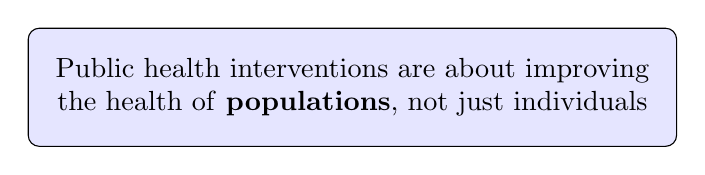
\begin{tikzpicture}
\node[draw, rounded corners, fill=blue!10, text width=8cm, align=center, minimum height=1.5cm] {
    Public health interventions are about improving\\
    the health of \textbf{populations}, not just individuals
};
\end{tikzpicture}
\end{center}
\end{frame}

\begin{frame}
\frametitle{Evaluation: Definition and Purpose}

% Customized block with lighter colors and no shadow
{\setbeamercolor{block title}{bg=blue!15,fg=black}
\setbeamercolor{block body}{bg=blue!5,fg=black}
\begin{block}{WHO Definition}
A \textbf{systematic way of learning from experience} to improve current activities and promote better planning
\end{block}}

\begin{itemize}[itemsep=0.3em]
    \item \textbf{Improve programs} and delivery systems
    \item \textbf{Guide resource allocation} with evidence
    \item \textbf{Continuous cycle}, not an afterthought
    \item Part of day-to-day management
\end{itemize}

\vspace{0.2cm}
\begin{center}
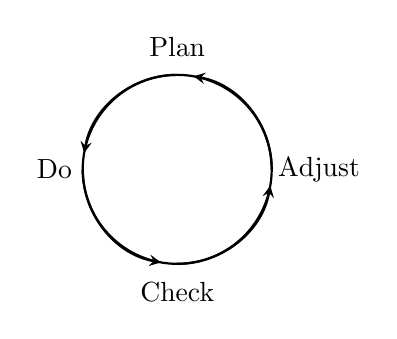
\begin{tikzpicture}[scale=1.2]
% Draw a complete circle first
\draw[thick] (0,0) circle (1);
% Add arrows on the circle
\draw[thick, ->, >=stealth] (1,0) arc (0:80:1);
\draw[thick, ->, >=stealth] (0,1) arc (90:170:1);
\draw[thick, ->, >=stealth] (-1,0) arc (180:260:1);
\draw[thick, ->, >=stealth] (0,-1) arc (270:350:1);
% Add labels outside the circle
\node at (0,1.3) {Plan};
\node at (-1.3,0) {Do};
\node at (0,-1.3) {Check};
\node at (1.5,0) {Adjust};
\end{tikzpicture}
\end{center}
\end{frame}

\section{Evaluability Assessment}

\begin{frame}
\frametitle{Evaluability Assessment}

% Customized block with lighter colors and no shadow
{\setbeamercolor{block title}{bg=blue!15,fg=black}
\setbeamercolor{block body}{bg=blue!5,fg=black}
\begin{block}{Key Question}
\textit{Is the program set up in a way that can be meaningfully evaluated?}
\end{block}}

% Removed vertical space to allow more room
\begin{columns}[t, totalwidth=\textwidth] % lowercase t for alignment, explicit total width
\column{0.46\textwidth} % Slightly reduced width for more space between columns
\textbf{Program factors:}
\begin{itemize}[itemsep=0.3em, leftmargin=1.5em] % Controlled spacing and margin
    \item Are goals clear and realistic?
    \item Is program theory plausible?
    \item Who will use evaluation results?
\end{itemize}

\column{0.46\textwidth} % Slightly reduced width for more space between columns
\textbf{Practical factors:}
\begin{itemize}[itemsep=0.3em, leftmargin=1.5em] % Controlled spacing and margin
    \item Time available
    \item Financial resources
    \item Available expertise
    \item Political buy-in
\end{itemize}
\end{columns}

% Added a little space at the bottom to balance the slide
\vspace{0.5cm}
\end{frame}

\section{Performance vs. Impact}

\begin{frame}
\frametitle{What to Measure: Performance vs. Impact}

\begin{columns}[t] % Top alignment
\column{0.47\textwidth}
\textbf{Performance Indicators}
\begin{itemize}[itemsep=0.2em] % Reduced spacing
    \item Program operations
    \item Service provision
    \item Utilization
    \item Coverage
    \item Quality
    \item Acceptability
\end{itemize}

\column{0.47\textwidth}
\textbf{Impact Indicators}
\begin{itemize}[itemsep=0.2em] % Reduced spacing
    \item Health improvements
    \item Disease reduction
    \item Equity effects
    \item Social justice
    \item Economic development
    \item Long-term outcomes
\end{itemize}
\end{columns}

\vspace{0.3cm}
% Customized block with lighter colors and no shadow
{\setbeamercolor{block title}{bg=blue!15,fg=black}
\setbeamercolor{block body}{bg=blue!5,fg=black}
\begin{block}{Data Sources}
\small
\begin{itemize}[itemsep=0.1em] % Even smaller spacing
    \item \textbf{Performance:} Program records, attendance logs, participant surveys
    \item \textbf{Impact:} Population health surveys, disease surveillance, economic data
\end{itemize}
\end{block}}
\end{frame}

\section{Levels of Certainty}

\begin{frame}
\frametitle{Levels of Certainty: How Confident Are We?}

% Customized block with lighter colors and no shadow
{\setbeamercolor{block title}{bg=blue!15,fg=black}
\setbeamercolor{block body}{bg=blue!5,fg=black}
\begin{block}{Key Question}
\textit{How confident can we be that the program caused the changes we see?}
\end{block}}

\vspace{0.2cm}
\begin{columns}[t] % Top alignment
\column{0.31\textwidth}
\textbf{Adequacy}
\begin{itemize}[itemsep=0.2em] % Reduced spacing
    \item Did program meet stated objectives?
    \item Compare results to targets
    \item Simplest level of certainty
\end{itemize}

\column{0.31\textwidth}
\textbf{Plausibility}
\begin{itemize}[itemsep=0.2em] % Reduced spacing
    \item Is it likely program caused change?
    \item Requires comparison
    \item Before/after or with/without
\end{itemize}

\column{0.31\textwidth}
\textbf{Probability}
\begin{itemize}[itemsep=0.2em] % Reduced spacing
    \item Statistical confidence
    \item Randomized Control Trials (RCTs)
    \item Highest level of certainty
\end{itemize}
\end{columns}
\end{frame}

\section{Key Evaluation Concepts}

\begin{frame}
\frametitle{Efficacy vs. Effectiveness vs. Efficiency}

\begin{columns}[t] % Top alignment
\column{0.31\textwidth}
\textbf{Efficacy}
\begin{itemize}[itemsep=0.2em] % Reduced spacing
    \item Does it work under ideal conditions?
    \item Controlled research setting
    \item Perfect implementation
    \item \textit{Potential}
\end{itemize}

\column{0.31\textwidth}
\textbf{Effectiveness}
\begin{itemize}[itemsep=0.2em] % Reduced spacing
    \item Does it work in the real world?
    \item Routine conditions
    \item Imperfect implementation
    \item \textit{Reality}
\end{itemize}

\column{0.31\textwidth}
\textbf{Efficiency}
\begin{itemize}[itemsep=0.2em] % Reduced spacing
    \item Resources vs. results
    \item Economic dimension
    \item Cost-effectiveness
    \item Requires effectiveness first
\end{itemize}
\end{columns}

\vspace{0.3cm}
% Customized alert block with lighter colors
{\setbeamercolor{block title alerted}{bg=red!20,fg=black}
\setbeamercolor{block body alerted}{bg=red!10,fg=black}
\begin{alertblock}{Example: Oral Contraceptives}
High efficacy in trials (perfect use) vs. lower effectiveness in communities (actual use)
\end{alertblock}}
\end{frame}

\section{Case Examples}

\begin{frame}
\frametitle{Example 1: Evaluating Smoking Bans}

\begin{columns}[t] % Top alignment with lowercase t
\column{0.48\textwidth}
\textbf{Performance Measures}
\begin{itemize}[itemsep=0.2em] % Reduced item spacing
    \item Implementation of ban
    \item Compliance by establishments
    \item Air quality measurements
    \item Public awareness
\end{itemize}

\vspace{0.2cm}
\textbf{Plausibility Check}
\begin{itemize}[itemsep=0.2em] % Reduced item spacing
    \item Compare trends in places with ban vs. without
    \item Control for other factors
\end{itemize}

\column{0.48\textwidth}
\textbf{Impact Measures}
\begin{itemize}[label=\textbullet, itemsep=0.2em] % Reduced item spacing
    \item Reduced exposure to secondhand smoke
    \item Smoking rates in population
    \item Smoking-related disease rates
    \item Hospital admissions
\end{itemize}
\end{columns}

% Image moved to bottom of frame with controlled size
\begin{center}

\includegraphics[width=0.45\textwidth]{tobacco.png}
\end{center}
\end{frame}

\begin{frame}
\frametitle{Example 2: Condom Use Programs for STI Prevention}

\begin{columns}[t] % Top alignment with lowercase t
\column{0.47\textwidth}
\textbf{Performance Measures}
\begin{itemize}[label=\textbullet, itemsep=0.2em] % Reduced item spacing
    \item Number of condoms distributed/sold
    \item Accessibility of condoms
    \item Self-reported condom use
    \item Knowledge about proper use
\end{itemize}

\vspace{0.2cm}
\textbf{Efficacy vs. Effectiveness}
\begin{itemize}[label=\textbullet, itemsep=0.2em] % Reduced item spacing
    \item Efficacy: High when used correctly
    \item Effectiveness: Depends on consistent proper use
\end{itemize}

\column{0.47\textwidth}
\textbf{Impact Measures}
\begin{itemize}[label=\textbullet, itemsep=0.2em] % Reduced item spacing
    \item STI rates in target population
    \item HIV infection rates
    \item Unintended pregnancy rates
\end{itemize}

\vspace{0.2cm}
\textbf{Key Insight}
\begin{itemize}[label=\textbullet, itemsep=0.2em] % Reduced item spacing
    \item Distribution alone isn't enough
    \item Behavior change required for impact
    \item Education component
\end{itemize}
\end{columns}

% Image moved to bottom with reduced size
\vspace{0.2cm}
\begin{center}

\includegraphics[width=0.4\textwidth]{condoms.jpg}
\end{center}
\end{frame}

\begin{frame}
\frametitle{Example 3: Urban Greenways for Active Transportation}

\begin{columns}[T]
\column{0.48\textwidth}
\textbf{Impact Measures}
\begin{itemize}[label=\textbullet, itemsep=0.2em]
    \item Physical activity and mobility
    \item Reductions in obesity and CVD rates
    \item Mental health and well-being outcomes
    \item Environmental benefits (air quality, heat)
    \item Traffic safety and injury rates
\end{itemize}

\column{0.48\textwidth}
\vspace{0.5cm}
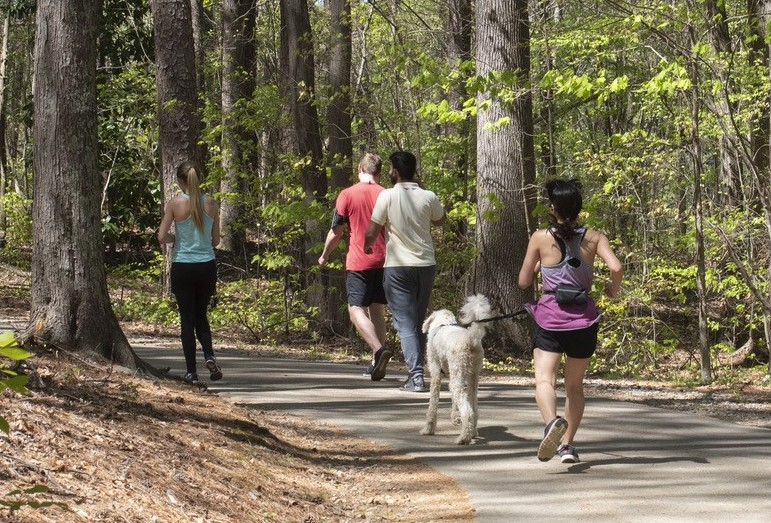
\includegraphics[width=\textwidth]{greeways.jpg}
\end{columns}
\end{frame}

\begin{frame}
\frametitle{Example 3: Urban Greenways - Community Use}
\begin{columns}[T]
\column{0.48\textwidth}
\textbf{Community Benefits}
\begin{itemize}[label=\textbullet, itemsep=0.2em]
    \item Multi-modal use (walking, cycling, running)
    \item Accessible to diverse populations
    \item Social connectivity and community building
    \item Cost-effective transportation alternative
    \item Enhanced quality of life
\end{itemize}

\column{0.48\textwidth}
\vspace{0.5cm}
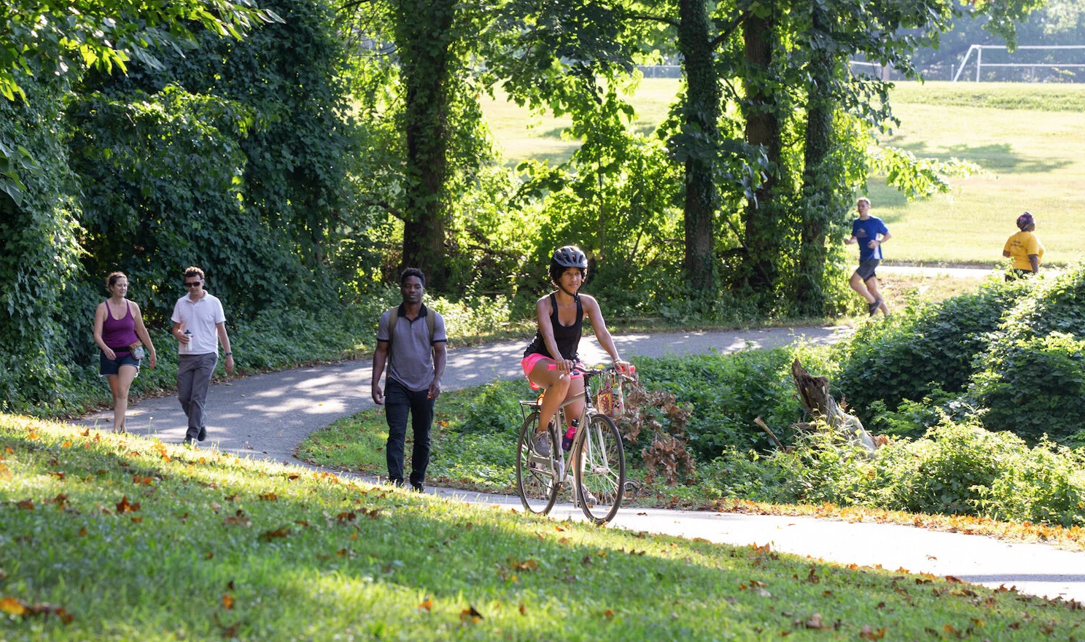
\includegraphics[width=\textwidth]{greewaysB.png}
\end{columns}
\end{frame}

\begin{frame}
\frametitle{Example 3: Urban Greenways - Safety Considerations}
\begin{columns}[T]
\column{0.48\textwidth}
\textbf{Safety Measures}
\begin{itemize}[label=\textbullet, itemsep=0.2em]
    \item Wildlife encounter protocols
    \item Emergency access and response
    \item Lighting and visibility
    \item User education and signage
    \item Regular maintenance and monitoring
\end{itemize}

\column{0.48\textwidth}
\vspace{0.5cm}
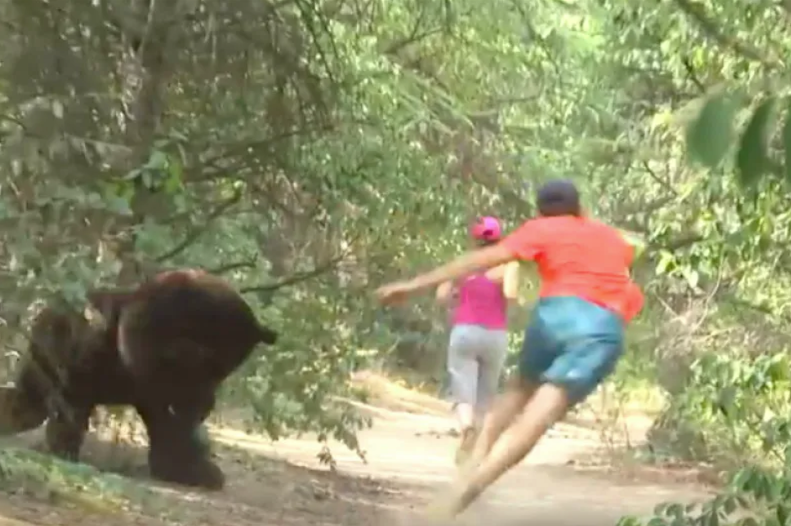
\includegraphics[width=\textwidth]{greewaysC.png}
\end{columns}
\end{frame}

\section{Economic Appraisal}

\begin{frame}
\frametitle{Economic Appraisal: Why It Matters}

% Customized alert block with lighter colors
{\setbeamercolor{block title alerted}{bg=red!20,fg=black}
\setbeamercolor{block body alerted}{bg=red!10,fg=black}
\begin{alertblock}{Resources Are Limited}
Public health budgets aren't infinite
\end{alertblock}}

% Customized block with lighter colors
{\setbeamercolor{block title}{bg=blue!15,fg=black}
\setbeamercolor{block body}{bg=blue!5,fg=black}
\begin{block}{Purpose}
\begin{itemize}[label=\textbullet, itemsep=0.2em] % Reduced spacing
    \item Compare costs and consequences of different options
    \item Help justify spending
    \item Prioritize interventions
    \item Make smart choices with scarce resources
\end{itemize}
\end{block}}

\vspace{0.2cm}
\begin{center}
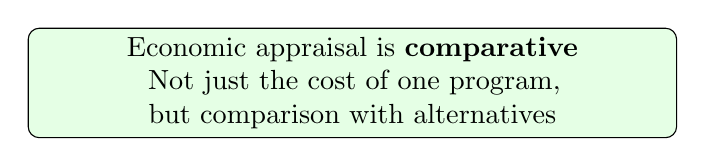
\begin{tikzpicture}
\node[draw, rounded corners, fill=green!10, text width=8cm, align=center, minimum height=1.2cm] {
    Economic appraisal is \textbf{comparative}\\
    Not just the cost of one program, but comparison with alternatives
};
\end{tikzpicture}
\end{center}
\end{frame}

\begin{frame}
\frametitle{Types of Economic Appraisal}

% Splitting information to avoid overcrowding
\begin{columns}[t] % Top alignment
\column{0.31\textwidth}
\textbf{Cost-Effectiveness Analysis (CEA)}
\begin{itemize}[itemsep=0.2em] % Reduced spacing
    \item Costs in money
    \item Outcomes in natural units
    \item E.g., cost per life saved
    \item E.g., cost per case prevented
\end{itemize}

\column{0.31\textwidth}
\textbf{Cost-Benefit Analysis (CBA)}
\begin{itemize}[itemsep=0.2em] % Reduced spacing
    \item Everything in monetary terms
    \item Includes healthcare savings
    \item Includes productivity gains
    \item Allows cross-sector comparison
\end{itemize}

\column{0.31\textwidth}
\textbf{Cost-Utility Analysis (CUA)}
\begin{itemize}[itemsep=0.2em] % Reduced spacing
    \item Specific type of CEA
    \item Outcomes in QALYs
    \item Combines length and quality of life
    \item Cost per QALY gained
\end{itemize}
\end{columns}

\vspace{0.3cm}
\begin{center}
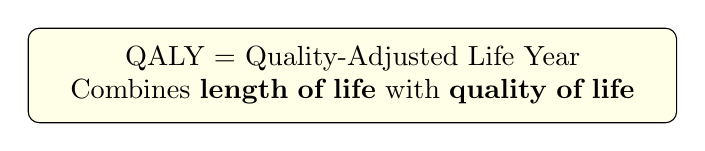
\begin{tikzpicture}
\node[draw, rounded corners, fill=yellow!10, text width=8cm, align=center, minimum height=1.2cm] {
    QALY = Quality-Adjusted Life Year\\
    Combines \textbf{length of life} with \textbf{quality of life}
};
\end{tikzpicture}
\end{center}
\end{frame}

\begin{frame}
\frametitle{Putting It All Together}

\begin{center}
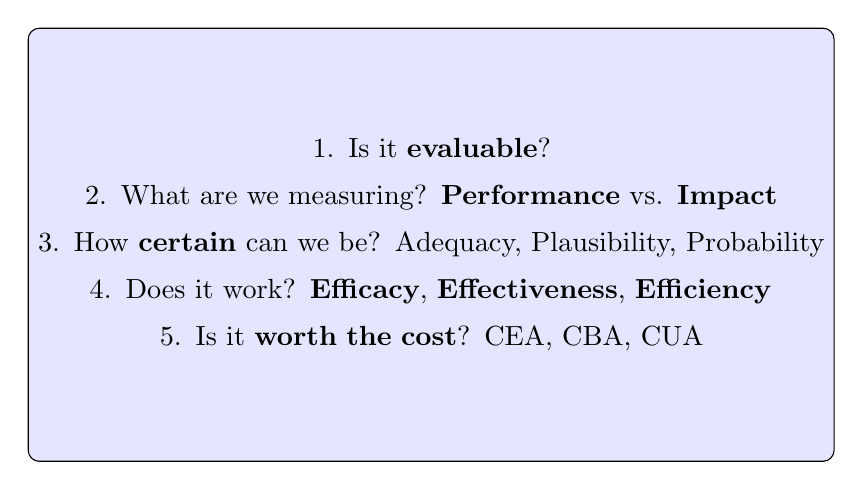
\begin{tikzpicture}
\node[draw, rounded corners, fill=blue!10, text width=10cm, align=center, minimum height=5.5cm] {
    1. Is it \textbf{evaluable}?\\[0.5em]
    2. What are we measuring? \textbf{Performance} vs. \textbf{Impact}\\[0.5em]
    3. How \textbf{certain} can we be? Adequacy, Plausibility, Probability\\[0.5em]
    4. Does it work? \textbf{Efficacy}, \textbf{Effectiveness}, \textbf{Efficiency}\\[0.5em]
    5. Is it \textbf{worth the cost}? CEA, CBA, CUA
};
\end{tikzpicture}
\end{center}

\vspace{0.2cm}

% Customized alert block with lighter colors
{\setbeamercolor{block title alerted}{bg=red!20,fg=black}
\setbeamercolor{block body alerted}{bg=red!10,fg=black}
\begin{alertblock}{Final Thought}
Think about a public health issue you know about. How might you apply these concepts to evaluate different approaches? What evidence would you need?
\end{alertblock}}
\end{frame}

\begin{frame}
\frametitle{Thank You}
\begin{center}
\Huge Thank You!\\
\vspace{1cm}
\normalsize
Questions \& Discussion
\end{center}
\end{frame}

\end{document}%%
